{\color{gray}\hrule}
\begin{center}
\section{American Vanilla Put Option Pricing}
\textbf{You can add small descriptions of what the current sections describe}
\bigskip
\end{center}
{\color{gray}\hrule}
\begin{multicols}{2}
\subsection{Problem Statement}
An American vanilla put option is more flexible than a European option because it can be exercised at any point before maturity or at maturity. This flexibility adds a complexity, as the pricing depends on deciding the best time to exercise based on the movement of the price of the underlying asset.

The Longstaff Schwartz approach is a practical method for pricing American options. It works by simulating multiple possible movements for the asset price and using regression techniques to figure out the optimal exercise strategy. The payoff at any point \textit{t} is:
\[\text{Payoff} = \max(0, K - S_t)
\]
where K is the strike price, and $S_t$ is the asset price at time t.
Our goal is to study how various factors like the number of simulated paths(N), the number of time steps(M), and the regression model affect the estimated option price. We also evaluate how efficient and accurate these methods are in practical applications.
\subsection{Methodology}
To price the American put option, we use the Longstaff-Schwartz Monte Carlo (LSM) method. This approach leverages regression techniques to estimate the continuation value at each step and determine the optimal exercise strategy.
\subsubsection{Simulation of Asset Prices}
Simulate \(N\) independent paths for the underlying asset price using the geometric Brownian motion (GBM) model:
\[
dS_t = (r - q) S_t \, dt + \sigma S_t \, dW_t,
\]
where \(dW_t\) represents the Wiener process.

Discretize the GBM equation using the time step \(\Delta t = \frac{T}{M}\) and simulate the price paths at each time step:
\[
S_{t+\Delta t} = S_t e^{(r - q - \frac{\sigma^2}{2}) \Delta t + \sigma \sqrt{\Delta t} Z},
\]
where \(Z \sim N(0,1)\) is a standard normal random variable.

\subsubsection{Payoff Calculation}
At each time step, calculate the payoff if the option is exercised immediately:
\[
\text{Payoff} = \max(0, K - S_t).
\]

\subsubsection{Regression for Continuation Value}
Starting from the second-to-last time step (\(t_{M-1}\)) and moving backward:
\begin{itemize}
    \item Use regression to estimate the continuation value of the option:
    \[
    \mathbb{E}[V_{t+1} \mid S_t],
    \]
    where \(V_{t+1}\) is the option value at the next time step.
    \item Fit a polynomial of degree \(K_{\text{reg}}\) (e.g., 2 or 3) to approximate the continuation value as a function of \(S_t\).
    \item Compare the continuation value with the immediate exercise value:
    \begin{itemize}
        \item If the immediate exercise value exceeds the continuation value, exercise the option.
        \item Otherwise, continue holding the option.
    \end{itemize}
\end{itemize}

\subsubsection{Discounting to Present Value}
For each path, calculate the discounted value of the option based on the optimal exercise strategy:
\[
V = e^{-rT} \cdot \text{Payoff}.
\]
Average these discounted values across all simulated paths to estimate the option price.

\subsubsection{Parameters Studied}
The following parameters are varied to analyze their impact on pricing accuracy and convergence:
\begin{itemize}
    \item \textbf{Sample size (\(N\)):} Increasing \(N\) reduces the stochastic error and stabilizes the price.
    \item \textbf{Number of time steps (\(M\)):} Larger \(M\) reduces time discretization error, improving accuracy.
    \item \textbf{Regression order (\(K_{\text{reg}}\)):} Affects the approximation of the continuation value.
\end{itemize}

\subsubsection{Binomial Black-Scholes with Richardson Extrapolation (BBSR)}
For American options, the Binomial Black-Scholes with Richardson Extrapolation (BBSR) method improves the accuracy of pricing American options by refining the standard binomial model. It works by using smaller time steps in the calculation and then applying extrapolation to estimate the option price as if the time steps were infinitely small. This reduces errors and gives highly accurate results. BBSR is especially helpful for American options because it can effectively handle the complexity of early exercise. Comparing these accurate results with those from the Longstaff-Schwartz method helps assess how affective the Monte Carlo method is.
\subsection{Results}

\subsubsection{Convergence Analysis for American Put Options}
The results demonstrate the impact of sample size (\(N\)), time steps (\(M\)), and regression order (\(K_{\text{reg}}\)) on the accuracy and stability of the Longstaff-Schwartz Monte Carlo (LSM) method for pricing American options.

\textbf{1. Effect of Sample Size (\(N\)):}  
As the number of simulated paths \(N\) increases, the estimated option price becomes progressively more stable and convergent (Figure 7).

\begin{itemize}
    \item At small \(N\) (e.g., \(N = 1,000\)), the option prices exhibit significant dispersion and volatility due to stochastic errors.
    \item As \(N\) increases to values like \(10,000\), the dispersion reduces, and prices cluster around the true value (approximately 2.22).
\end{itemize}
This highlights the importance of sufficient sample size to average out randomness and achieve stable results.

\textbf{2. Effect of Time Steps (\(M\)):}  
Time discretization plays a crucial role in pricing accuracy (Figure 8).

\begin{itemize}
    \item When \(M\) is small (e.g., \(M < 1,000\)), time discretization errors lead to significant volatility, especially for smaller \(N\).
    \item As \(M\) increases (e.g., \(M \geq 3,000\)), the prices stabilize, reducing variability and improving accuracy.
\end{itemize}
The convergence trend becomes clear when both \(N \geq 3,000\) and \(M \geq 2,000\), where the results stabilize within a narrow range (2.2 to 2.3).

\textbf{3. Effect of Regression Order (\(K_{\text{reg}}\)):}  
The regression order in the LSM method impacts the approximation of continuation values (Figure 5).
\end{multicols}
\begin{figure}
    \centering
    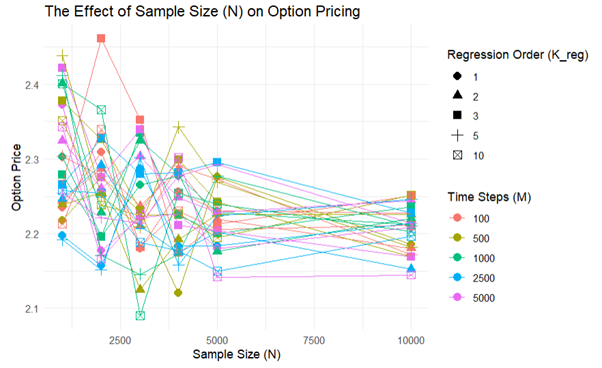
\includegraphics[width=0.9\linewidth]{Picture1.png}
    \caption{Option Price - Sample Size}
    \label{fig:enter-label}
\end{figure}
\begin{figure}
    \centering
    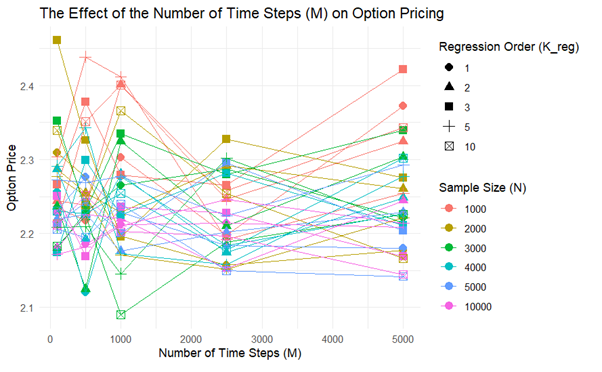
\includegraphics[width=0.9\linewidth]{Picture2.png}
    \caption{Option Price - Time Steps}
    \label{fig:enter-label}
\end{figure}

\begin{figure}[H]
    \centering
    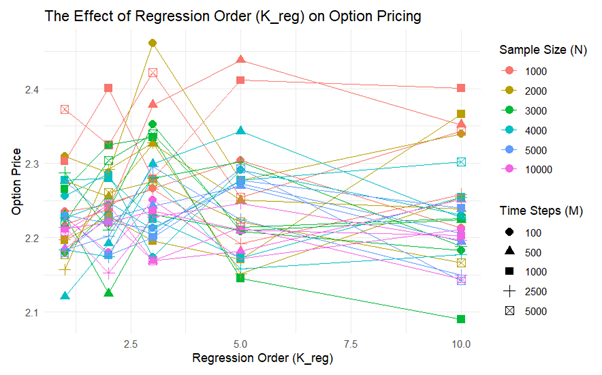
\includegraphics[width=0.9\linewidth]{Picture3.png}
    \caption{Option Price - Regression Order}
    \label{fig:enter-label}
\end{figure}
\begin{multicols}{2}
\begin{itemize}
    \item \textbf{Low Regression Orders (\(K_{\text{reg}} \leq 3\)):} These provide stable and reliable results, particularly for larger \(N\) (e.g., \(N = 5,000\)).
    \item \textbf{High Regression Orders (\(K_{\text{reg}} \geq 5\)):} These can lead to instability due to overfitting, especially when \(N\) is small or \(M\) is sparse.
\end{itemize}
For practical purposes, a regression order of \(K_{\text{reg}} = 2 \sim 3\) offers a good balance between accuracy and stability.

\subsubsection{Comparison of LSM and BBSR Methods}
The comparison between the Longstaff-Schwartz Monte Carlo (LSM) method and the Binomial Black-Scholes with Richardson Extrapolation (BBSR) method reveals the following insights(Figure 9).
\end{multicols}
\begin{table}[h!]
\centering
\caption{Comparison of LSM and BBSR Prices for Various Parameters}
\begin{tabular}{|p{1.5cm}|p{1.5cm}|p{1.5cm}|p{2.5cm}|p{2.5cm}|}
\hline
\textbf{\(N\)} & \textbf{\(M\)} & \textbf{\(K_{\text{reg}}\)} & \textbf{LSM Price} & \textbf{BBSR Price} \\ \hline
1,000  & 100  & 2 & 2.16602 & 2.215176 \\ \hline
1,000  & 100  & 3 & 2.347223 & 2.215176 \\ \hline
1,000  & 100  & 5 & 2.312833 & 2.215176 \\ \hline
1,000  & 500  & 2 & 2.156658 & 2.223767 \\ \hline
1,000  & 500  & 3 & 2.211544 & 2.223767 \\ \hline
1,000  & 500  & 5 & 2.205814 & 2.223767 \\ \hline
1,000  & 1000 & 2 & 2.209214 & 2.224865 \\ \hline
1,000  & 1000 & 3 & 2.209717 & 2.224865 \\ \hline
1,000  & 2500 & 2 & 2.25208  & 2.225478 \\ \hline
\end{tabular}
\label{tab:LSM_vs_BBSR_1}
\end{table}
\begin{multicols}{2}

\textbf{1. Stability of the BBSR Method:}  
The BBSR method produces highly stable option prices, even for small \(N\) and \(M\), with prices consistently within a narrow range (approximately 2.215 to 2.225). This highlights its superior accuracy and makes it a reliable benchmark.
\end{multicols}
\begin{table}[h!]
\centering
\caption{Comparison of LSM and BBSR Prices for Larger Sample Sizes}
\begin{tabular}{|p{1.5cm}|p{1.5cm}|p{1.5cm}|p{2.5cm}|p{2.5cm}|}
\hline
\textbf{\(N\)} & \textbf{\(M\)} & \textbf{\(K_{\text{reg}}\)} & \textbf{LSM Price} & \textbf{BBSR Price} \\ \hline
10,000 & 100  & 2 & 2.25674 & 2.215176 \\ \hline
10,000 & 100  & 3 & 2.18681 & 2.215176 \\ \hline
10,000 & 100  & 5 & 2.22371 & 2.215176 \\ \hline
10,000 & 500  & 2 & 2.20556 & 2.223767 \\ \hline
10,000 & 500  & 3 & 2.215695 & 2.223767 \\ \hline
10,000 & 500  & 5 & 2.219789 & 2.223767 \\ \hline
10,000 & 1000 & 2 & 2.224479 & 2.224865 \\ \hline
10,000 & 1000 & 3 & 2.230177 & 2.224865 \\ \hline
10,000 & 2500 & 2 & 2.263049 & 2.225478 \\ \hline
\end{tabular}
\label{tab:LSM_vs_BBSR_2}
\end{table}

\begin{multicols}{2}
\textbf{2. Convergence of the LSM Method:}  
The LSM method shows more volatility for small \(N\) (e.g., \(N = 1,000\)) and small \(M\) (e.g., \(M = 100\)). However, as \(N\) and \(M\) increase:
\begin{itemize}
    \item LSM prices converge toward the BBSR benchmark.
    \item The scatter observed at smaller \(N\) and \(M\) reduces, with results stabilizing around the true option price.
\end{itemize}
\subsection{Discussion}
The results of pricing the American put option using the Longstaff-Schwartz Monte Carlo (LSM) method and the Binomial Black-Scholes with Richardson Extrapolation (BBSR) method highlight important findings regarding accuracy, convergence, and computational efficiency.

\subsubsection{Stability and Accuracy of the BBSR Method}
The BBSR method consistently produced stable and accurate option prices, even with smaller time steps (\(M\)) and sample sizes (\(N\)). We assume this stability is caused by its ability to improve results using Richardson extrapolation, which effectively eliminates discretization errors i.e errors caused due to the discrete approximation of a continuous process. In all cases, the BBSR prices remained within a narrow range of approximately 2.215 to 2.225, making it really useful for evaluating the LSM method.

\textbf{The key advantages of the BBSR method include:}
\begin{itemize}
    \item \textbf{High Accuracy:} Prices are consistently close to the true option value.
    \item \textbf{Reduced Sensitivity:} Results are less affected by changes in \(N\) which \(M\), makes the method computationally efficient for smaller datasets.
    \item \textbf{Ease of Implementation:} The method provides reliable estimates without requiring approximations from the regression model in the LSM method.
\end{itemize}
However, the BBSR method is limited to simpler models and may not generalize as effectively for more complex derivatives which can have higher number of dependencies.

\subsubsection{Convergence and Efficiency of the LSM Method}
The Longstaff-Schwartz method showed strong performance, particularly for larger \(N\) and \(M\), while converging to the BBSR values. However, the results show that LSM is sensitive to a few key parameters:

\textbf{Sample Size (\(N\)):}  
\begin{itemize}
    \item At smaller values of \(N\) (e.g., \(N = 1,000\)), the option prices had significant volatility, reflecting the stochastic nature of Monte Carlo simulations.
    \item As \(N\) increased, the random noise reduced, and the prices stabilized close to the benchmark (e.g., \(N = 10,000\)).
\end{itemize}

\textbf{Number of Time Steps (\(M\)):}  
\begin{itemize}
    \item Time discretization errors were observed for smaller \(M\) (e.g., \(M = 100\)).
    \item Increasing \(M\) (e.g., \(M \geq 1,000\)) reduced these errors, improving the accuracy of the continuation value approximation.
\end{itemize}

\textbf{Regression Order (\(K_{\text{reg}}\)):}  
\begin{itemize}
    \item For \(K_{\text{reg}} \leq 3\), the LSM method provided stable and accurate estimates.
    \item Higher regression orders (\(K_{\text{reg}} \geq 5\)) led to overfitting, particularly for smaller \(N\), introducing unnecessary variability.
    \item A regression order of \(K_{\text{reg}} = 2\) or \(3\) strikes the best balance between accuracy and computational efficiency.
\end{itemize}

\subsubsection{Computational Performance and Tradeoffs}
The BBSR method is computationally efficient for small datasets but becomes resource-intensive as time steps increase. The LSM method, while computationally heavier due to the need for multiple regressions, offers flexibility in handling early exercise features and complex models.

\textbf{The following tradeoffs are observed:}
\begin{itemize}
    \item \textbf{Accuracy vs. Computational Cost:}  
    While the LSM method requires a larger \(N\) and \(M\) to converge, the compute time increases significantly. For practical purposes, values such as \(N = 10,000\) and \(M = 1,000\) are recommended for balancing accuracy and efficiency.
    
    \item \textbf{Regression Complexity:}  
    Higher regression orders provide diminishing returns and increase compute time without significant improvements in the accuracy.
\end{itemize}

\subsubsection*{4. Practical Recommendations}
\begin{itemize}
    \item For applications where accuracy is critical and computational resources are limited, the BBSR method should be selected due to its stability.
    \item The Longstaff-Schwartz method is well-suited for scenarios requiring flexibility in handling path-dependent options or early exercise features. 
    \item Future improvements can include combining the LSM method with variance reduction techniques such as antithetic variates or control variates to further reduce variability and compute cost.
\end{itemize}

\subsubsection{Future Directions}
\begin{itemize}
    \item \textbf{Variance Reduction:} Implement variance reduction techniques (e.g., antithetic variates, control variates, stratified sampling) to enhance the efficiency of the LSM method.
    \item \textbf{Parallelization:} Use parallel computing to accelerate Monte Carlo simulations, particularly for large sample sizes.
    \item \textbf{Comparison with Other Methods:} Compare the LSM and BBSR methods with other techniques like Finite Difference Methods (FDM) or Quasi-Monte Carlo methods to analyze their accuracy and efficiency further.
    \item \textbf{Complex Derivatives:} Extend the analysis to other path-dependent options, such as barrier options or options with stochastic volatility.
\end{itemize}

The BBSR method serves as a stable and accurate benchmark for pricing American options, while the Longstaff-Schwartz method provides flexibility at the cost of higher computational requirements. The choice of method depends on the tradeoff between computational efficiency and model complexity. By optimizing sample size, time steps, and regression parameters, the LSM method can achieve results close to the BBSR benchmark while maintaining computational feasibility.
\end{multicols}